\capitulo{3}{Conceptos teóricos}

En este apartado se presentan los conceptos teóricos fundamentales tanto del ámbito tecnológico como biomédico. Además, se incluye una revisión del estado del arte centrada en la segmentación del cerebro fetal mediante técnicas de \textit{deep learning}. 

\section{Inteligencia Artificial y Machine Learning}
\subsection{Inteligencia Artificial}
La Inteligencia Artificial (IA) es una rama de la informática que trata de desarrollar sistemas capaces de realizar tareas que tradicionalmente han requerido inteligencia humana, como el reconocimiento de patrones, la toma de decisiones o la resolución de problemas. Su principal objetivo es dotar a las máquinas de la capacidad de aprender y adaptarse a nuevas situaciones sin intervención humana directa \cite{russell2010ia}.

\subsection{Machine Learning}
El aprendizaje automático o \textit{Machine Learning} (ML) es un subcampo de la IA basado en el desarrollo de algoritmos capaces de aprender a partir de datos. Estos algoritmos identifican patrones y relaciones dentro de los datos para realizar tareas de clasificación, regresión y agrupamiento. Se basan en modelos matemáticos que ajustan sus parámetros internos en función de los ejemplos previamente observados, con el objetivo de generalizar su comportamiento a nuevos casos no vistos \cite{mitchell1997ml}.

En base al tipo de entrenamiento que reciben, los algoritmos de ML se clasifican principalmente en tres categorías \cite{mitchell1997ml}:
\begin{itemize}
    \item \textbf{Aprendizaje supervisado}: el modelo se entrena con un conjunto de datos etiquetados, es decir, cada entrada va acompañada de su salida deseada. 
    \item \textbf{Aprendizaje no supervisado}: el modelo busca estructuras o patrones ocultos entre datos no etiquetados.
    \item \textbf{Aprendizaje por refuerzo}: el sistema aprende a tomar decisiones a través de la iteración con un entorno, optimizando una recompensa acumulada a lo largo del tiempo. 
\end{itemize} 
En el aprendizaje automático tradicional, gran parte del trabajo se centra en el preprocesamiento de los datos y la selección manual de características relevantes, proceso conocido como \textit{feature engineering} \cite{ng2020yearning}. Esta fase puede limitar la capacidad del modelo para reconocer relaciones más complejas en los datos.

\section{Deep Learning}
El aprendizaje profundo o \textit{Deep Learning} (DL) es un área del aprendizaje automático basada en el uso de redes neuronales artificiales con múltiples capas ocultas. Su objetivo es permitir que las máquinas aprendan automáticamente representaciones y patrones complejos a partir de grandes cantidades de datos, sin necesidad de que un programador defina explícitamente las características a extraer.

Una de las principales fortalezas del DL es su capacidad de aprender representaciones jerárquicas de los datos. En sus primeras capas detecta patrones simples, y en capas más profundas combina estas representaciones para identificar conceptos complejos.

La eficacia del DL en los últimos años se ha visto impulsada por la disponibilidad de grandes volúmenes de datos, gracias al \textit{Big Data}, y por el uso de hardware especializado, como \textit{GPUs} (Unidades de Procesamiento Gráfico) o \textit{TPUs} (Unidades de Procesamiento Tensorial), que permiten procesar grandes cantidades de información de manera eficiente \cite{deeplearning2016}. 

\subsection{Segmentación de imágenes}
La segmentación de imágenes es una técnica fundamental en visión por computador. Consiste en dividir una imagen en múltiples regiones o segmentos, donde cada región agrupa píxeles que comparten ciertas características, como color o textura.

Como resultado, permite identificar y aislar objetos o áreas específicas dentro de una imagen, facilitando su análisis automático. 

\subsubsection{Segmentación por instancias}
Este tipo de segmentación no solo clasifica cada píxel con una etiqueta de clase, sino que también diferencia entre distintas instancias de un mismo objeto. Es decir, identifica y separa objetos individuales, incluso si pertenecen a la misma categoría. \cite{klinger2023segmentacion}

En el caso de este proyecto, se emplea este tipo de segmentación, ya que permite que la red neuronal aprenda a delimitarlas con precisión en cada imagen médica, además de clasificar regiones automáticamente. Esto es esencial en aplicaciones clínicas y de diagnóstico.

\section{Redes Neuronales Artificiales}
Las redes neuronales artificiales o \textit{Artificial Neural Networks} (ANN) son modelos computacionales inspirados en el funcionamiento del cerebro humano, en particular, en el modo en que las neuronas del cerebro procesan y transmiten la información \cite{ann2004}. Se diseñan con el objetivo de que aprendan automáticamente, siendo capaces de reconocer patrones, realizar clasificaciones o aproximar funciones no lineales a partir de datos \cite{deeplearning2016}.

Las neuronas artificiales se organizan en capas \cite{ann2004}:
\begin{itemize}
    \item Capa de entrada: recibe los datos de entrada del sistema, como las imágenes.
    \item Capas ocultas: una o varias capas intermedias que procesan información mediante conexiones ponderadas.
    \item Capa de salida: proporciona la respuesta final del modelo, como la máscara de segmentación.
\end{itemize}
Cada conexión entre neuronas tiene asociado un peso que determina la importancia de la señal transmitida. Las neuronas aplican una función de activación a la suma ponderada de sus entradas, lo que introduce no linealidades y permite modelar las relaciones complejas \cite{deeplearning2016}.

El proceso de aprendizaje de estas redes se basa principalmente en dos fases \cite{deeplearning2016}:
\begin{itemize}
    \item \textbf{Propagación hacia adelante (forward propagation)}: los datos se transmiten desde la capa de entrada hasta la salida, generando una predicción.
    \item \textbf{Retropropagación del error (\textit{backpropagation})}: se calcula el error entre la predicción obtenida y la salida deseada, y este error se propaga en sentido inverso a través de la red, actualizando los pesos mediante algoritmos de optimización.
\end{itemize}

A través de múltiples iteraciones de este proceso, la red ajusta sus parámetros internos para mejorar progresivamente su rendimiento y aprender a generalizar a partir de ejemplos.

\subsection{Redes Neuronales Convolucionales (CNN)}
Las redes neuronales convolucionales o \textit{Convolutional Neural Networks} (CNN) son una arquitectura específica de redes neuronales profundas, ampliamente utilizadas para tareas de procesamiento de imágenes, como clasificación, detección de objetos y segmentación \cite{gu2018cnn}. A diferencia de las redes tradicionales, las CNN están diseñadas específicamente para aprovechar la estructura espacial de los datos de entrada, lo que las hace especialmente eficaces en visión por computador \cite{ibmcnn}. 

La CNN típica consta de varias capas, cada una con un propósito específico en el proceso de extracción y aprendizaje de características:  
\begin{itemize}
    \item Capa de convolución: esta capa utiliza filtros o kernels que se deslizan sobre la imagen de entrada para extraer características locales, como bordes, texturas o patrones. Cada filtro está diseñado para responder a características específicas. Se puede destacar que, al aplicar varios filtros, la red aprende a detectar una gran variedad de rasgos relevantes para la tarea \cite{sotil2022cnn}.
    \item Funciones de activación: son funciones no lineales que se aplican a la salida de cada neurona para introducir no linealidad en el modelo, permitiendo así aprender relaciones complejas. Algunas de las funciones más comunes son:
    \begin{itemize}
    \item \texttt{ReLU} (Unidad Lineal Rectificada): activa solo los valores positivos, ayudando a evitar problemas de saturación y acelerando el entrenamiento \cite{ibmcnn}. 
    \item  TanH (Tangente hiperbólica): escala la salida entre -1 y 1, útil en ciertos contextos pero puede sufrir problemas de saturación \cite{deeplearning2016}.
    \item Sigmoide: transforma la salida en un valor entre 0 y 1, especialmente útil para tareas de clasificación binaria, aunque también puede saturarse y ralentizar el aprendizaje \cite{deeplearning2016}.
    \end{itemize}
    \item Capa de Agrupación (Pooling): la función principal de esta capa es reducir la dimensionalidad de las representaciones obtenidas en las capas anteriores, facilitando el manejo de la información y reduciendo el costo computacional. Los dos métodos comunes son \cite{ibmcnn, ajmal2018cnn}:
    \begin{itemize}
        \item Max pooling: selecciona el valor máximo en cada región, conservando las características más importantes.
        \item Average pooling: calcula el promedio de los valores, proporcionando una visión más general de la información en esa región.
    \end{itemize}
\end{itemize}

El flujo jerárquico de las CNN permite que las primeras capas detecten características simples, mientras que las capas más profundas combinan estas representaciones para reconocer estructuras complejas. Esto es especialmente útil en tareas de segmentación médica, donde es necesario identificar con precisión regiones anatómicas específicas dentro de imágenes complejas. 

La Figura \ref{fig:cnn_arquitectura} muestra el flujo jerárquico típico de una CNN, desde la imagen de entrada, pasando por múltiples capas de convolución y agrupación, hasta llegar a una capa completamente conectada que realiza la predicción final.

\begin{figure}[h]
    \centering
    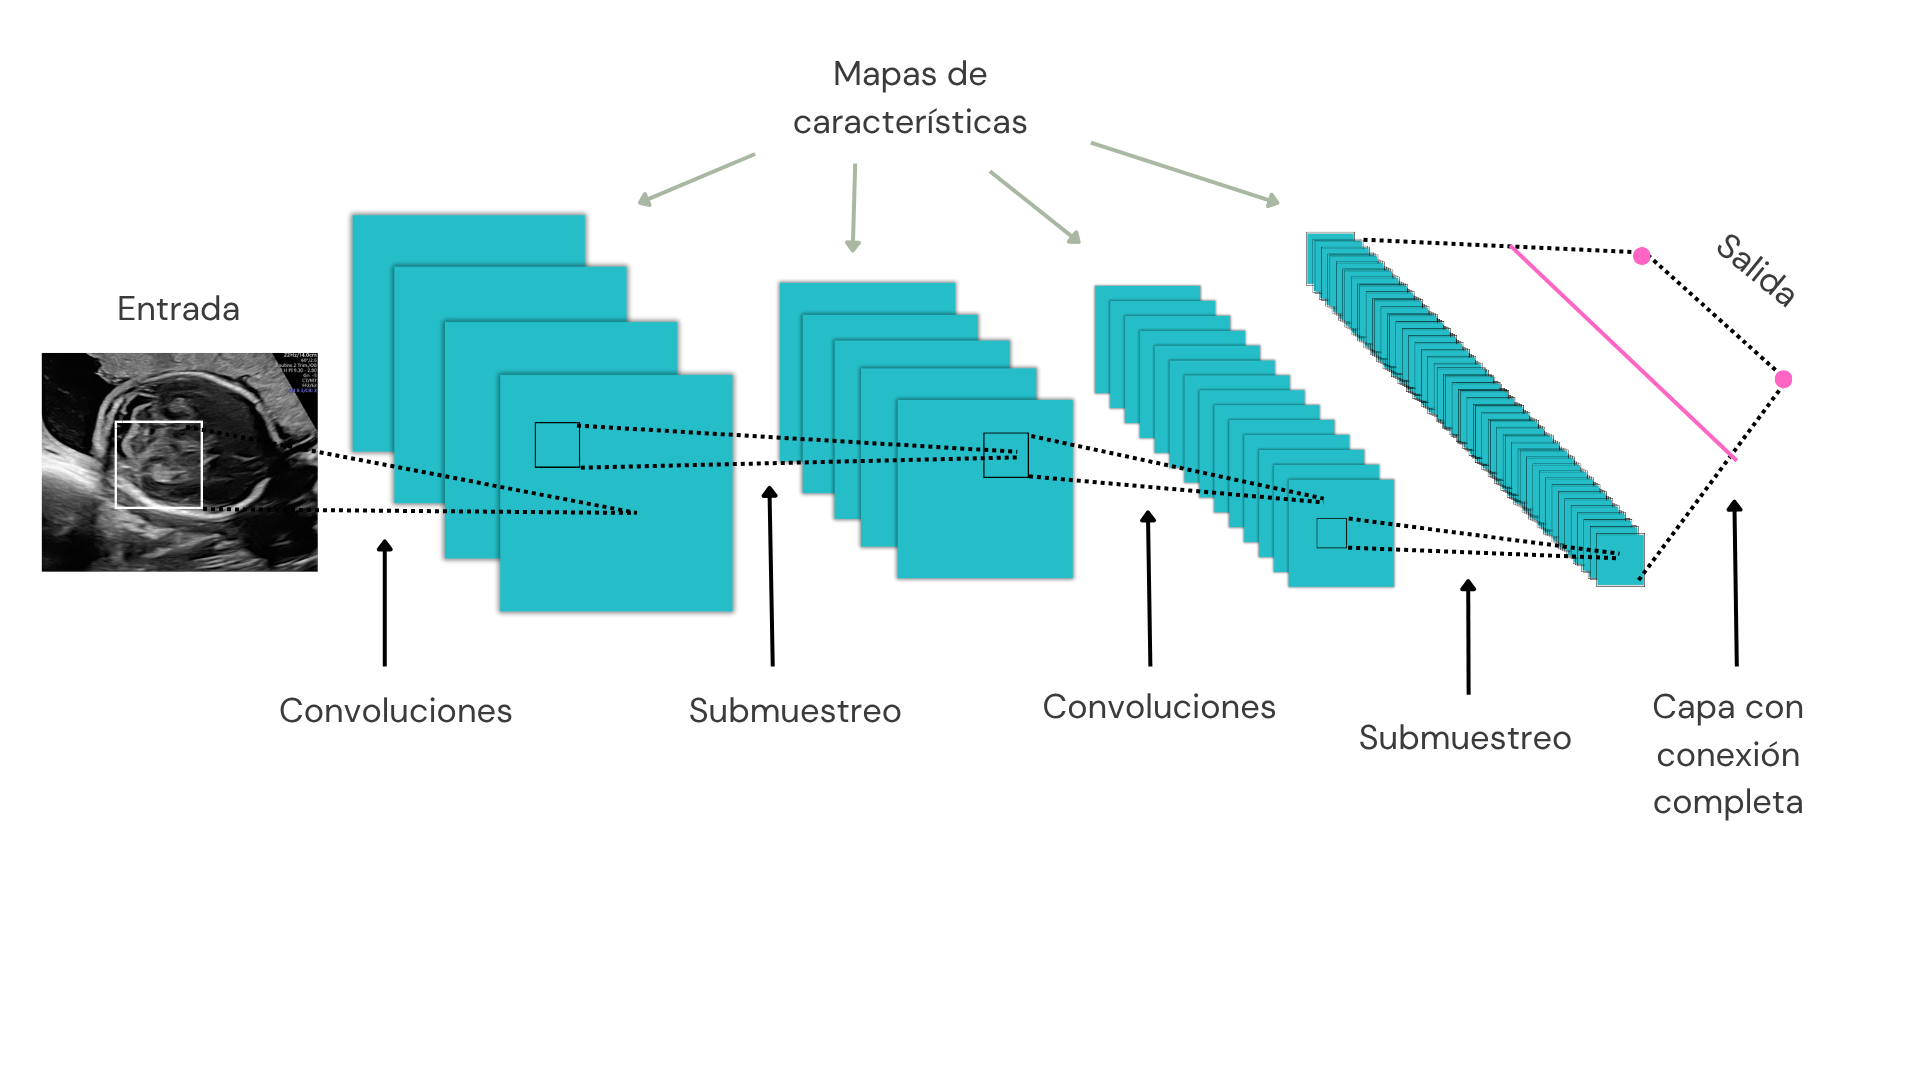
\includegraphics[width= \textwidth]{img/cnn.png}
    \caption{Arquitectura típica de una red neuronal convolucional (CNN). Imagen adaptada de Marcos Esparza Arizpe \cite{cnnimagen}}
    \label{fig:cnn_arquitectura}
\end{figure}

En comparación, las ANN tradicionales utilizan conexiones totalmente conectadas que no distinguen la posición relativa de los datos. Las CNN, en cambio, preservan esta estructura espacial, permitiendo detectar patrones locales específicos. Este enfoque las hace considerablemente más eficaces para tareas como la segmentación de estructuras cerebrales en imágenes fetales \cite{ajmal2018cnn}.


\section{Ecografía}
La ecografía, o ultrasonido médico, es una técnica de imagen que utiliza ondas acústicas de alta frecuencia (normalmente entre 2-10 MHz en diagnóstico fetal) para obtener imágenes de las estructuras internas del cuerpo humano sin necesidad de procedimientos invasivos. Estas ondas se emiten y reciben como ondas mecánicas longitudinales que se propagan a través de los tejidos, reflejándose en las interfaces entre distintos materiales en función de su impedancia acústica \cite{leigthon2007ultrasound}.

Desde un punto de vista físico, el ultrasonido representa una forma de energía mecánica que se transmite en forma de ondas de compresión y rarefacción. Estas ondas generan oscilaciones en las partículas del medio sin producir un desplazamiento neto, permitiendo así el transporte de energía sin transferencia de materia. Este principio físico es lo que permite que esta técnica produzca imágenes en tiempo real \cite{leigthon2007ultrasound, ultrasonido}.

Gracias a estas características, se ha convertido en una herramienta ideal para aplicaciones médicas, especialmente en el campo de la obstetricia. Su carácter seguro, no invasivo y en tiempo real la hace fundamental para observar el desarrollo del feto y detectar posibles anomalías durante la gestación \cite{leigthon2007ultrasound}. 

\subsection{Ecografías 2D}
La ecografía bidimensional (2D) es la modalidad más ampliamente utilizada para representar las imágenes obtenidas mediante ultrasonido. En este tipo de ecografía, el transductor genera un barrido, ya sea mecánico o electrónico, de una sección del cuerpo. Las ondas de ultrasonido reflejadas son procesadas para producir una imagen plana que representa un corte transversal de los tejidos analizados \cite{ultrasonido}.

En el contexto del diagnóstico prenatal, las ecografías 2D permiten una visualización detallada de las estructuras anatómicas del feto, entre ellas el cerebro. Estas imágenes son esenciales para evaluar el crecimiento fetal y posibles anomalías estructurales. Además, presentan ventajas como su alta disponibilidad, relativa simplicidad técnica y bajo coste, lo que las hace accesibles para una amplia gama de aplicaciones clínicas \cite{2dultrasound}.

\section {Cerebelo fetal}
El cerebelo presenta un papel fundamental en el desarrollo neurológico, contribuyendo a funciones motoras, cognitivas y emocionales \cite{schmahmann1998cerebellum}. La evaluación de sus estructuras anatómicas resulta crucial para identificar anomalías en su desarrollo. A continuación, se describen las partes clave del cerebelo.
\subsection{Vermis cerebeloso}
El vermis cerebeloso constituye la parte central del cerebelo, encargado de conectar sus dos hemisferios. Es fundamental en el control del equilibrio, la postura y la coordinación motora. Además, está implicado en funciones cognitivas y emocionales debido a sus conexiones con regiones del cerebro como la corteza prefrontal y el sistema límbico \cite{wolf2009vermis}. En la Figura \ref{fig: parte_anatomicas_cerebelo}, el vermis está marcado en color rosa.

Alteraciones en su desarrollo, como la hipoplasia, se asocian a síndromes neurológicos, entre los que destacan el síndrome de Dandy-Walker \cite{dandy2023} y ciertas formas de ataxia.

\subsection{Cisterna magna}
La cisterna magna o cisterna cerebelomodular es la mayor de las cisternas subaracnoideas del sistema nervioso central. Se localiza entre la superficie inferior del cerebelo y facilita la circulación del líquido cefalorraquídeo (LCR), permitiendo su circulación desde el cuarto ventrículo hacia el espacio subaracnoideo que rodea el encéfalo y la médula espinal \cite{patel2023cisternamagna}. En la Figura \ref{fig: parte_anatomicas_cerebelo}, la cisterna aparece en color amarillo.

Alteraciones en su desarrollo, como la dilatación excesiva, pueden asociarse a diversas malformaciones cerebelosas, como el síndrome de Dandy-Walker y la mega cisterna magna. Estas patologías suelen estar interrelacionadas ya que la ausencia de vermis o hipoplasia del vermis cerebeloso puede generar un agrandamiento anómalo del espacio subaracnoideo, dando lugar a una cisterna magna \cite{patel2023cisternamagna}.

\subsection{Hemisferios cerebelosos}
Los hemisferios cerebelosos constituyen las regiones laterales del cerebelo y se encuentran separados por el vermis. Estas estructuras, junto con la cisterna magna, forman parte del plano transcebeloso evaluado en la ecografía prenatal. Cada hemisferio se divide en lóbulos y lobulillos, cuya corteza se organiza en capas que participan en la coordinación motora y el aprendizaje de movimientos \cite{kenhub}. En la Figura \ref{fig: parte_anatomicas_cerebelo}, los hemisferios cerebelosos están marcados en color morado.


Durante el desarrollo fetal, los hemisferios cerebelosos se expanden lateralmente desde los labios rómbicos, formando el cerebelo. Alteraciones en su desarrollo, como la hipoplasia cerebelosa, pueden comprometer la coordinación motora y otras funciones neurológicas \cite{volpecerebelo}.

\begin{figure}[h]
    \centering
    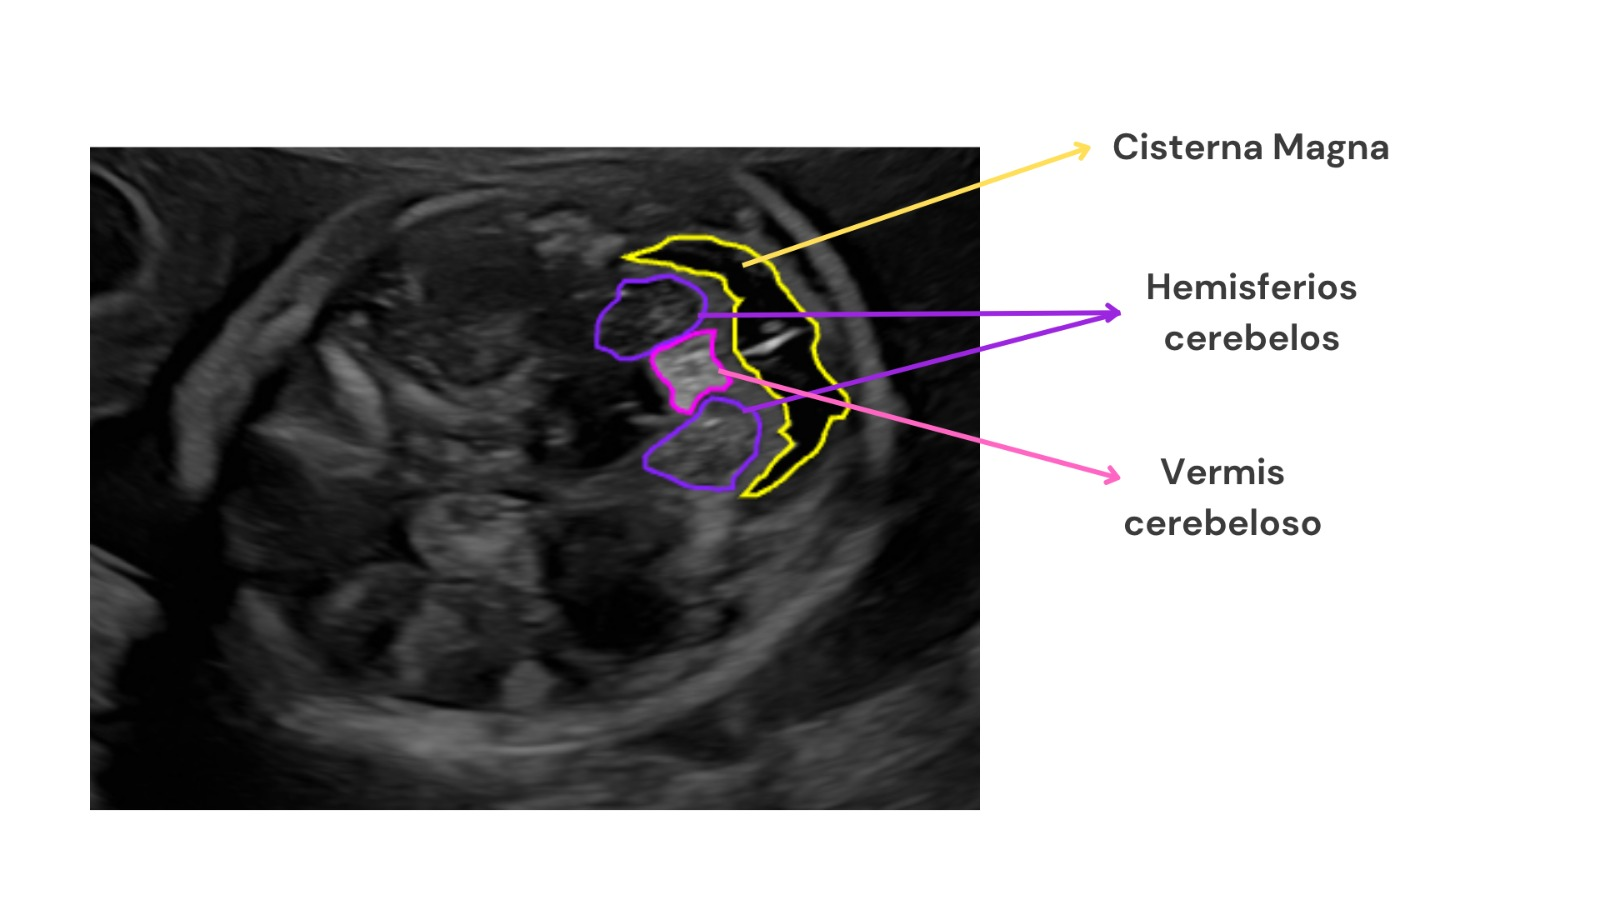
\includegraphics[width=\textwidth]{img/estructuras_interes.jpeg}
    \caption{Localización de las partes claves del cerebelo. Realización propia.}
    \label{fig: parte_anatomicas_cerebelo}
\end{figure}

\section{Estado del arte y trabajos relacionados}
La búsqueda de artículos e investigaciones relacionadas con el proyecto se ha realizado empleando buscadores científicos como \textit{PubMed}, \textit{Google Scholar}, \textit{Web of Science} y \textit{Nature}. A continuación, se exponen los estudios más relevantes encontrados en el ámbito de la segmentación de imágenes médicas mediante técnicas de DL, con especial atención a la aplicación en estructuras cerebrales fetales y análisis de imágenes de ultrasonido.

En el contexto del desarrollo prenatal humano, la detección y análisis temprano de estructuras como el cerebelo fetal es de vital importancia, dada su implicación en el desarrollo neurológico \cite{volpe2009, koning2017impacts}. Para abordar la complejidad inherente a las imágenes de ultrasonido y la variabilidad anatómica, diversos estudios han explorado la aplicación de Redes Neuronales Convolucionales (CNN) y arquitecturas avanzadas de segmentación basadas en DL \cite{hesamian2019}.

A nivel más general, diferentes revisiones han sintetizado los avances más relevantes en el uso de CNN para la segmentación de imágenes médicas \cite{hesamian2019, ajmal2018cnn}. Estos trabajos destacan la eficacia de arquitecturas como U-Net, ampliamente utilizadas por su capacidad para preservar tanto el contexto global como los detalles espaciales en tareas clínicas complejas.

Además, existen ejemplos de aplicación técnica como el presentado por Plain Concepts \cite{plain2021}, donde se describe el uso de modelos inspirados en \texttt{U-Net} para la segmentación precisa de órganos en diversas modalidades de imagen médica. Este tipo de contribuciones demuestra el potencial del aprendizaje profundo en entornos clínicos reales, complementando la evidencia académica.

En conjunto, estos trabajos proporcionan una base sólida para el presente proyecto, al evidenciar los avances en segmentación automatizada y su aplicación específica al análisis de imágenes médicas.

